
La cuantificaci\'on de {informaci\'on dada por la Ec. \ref{eq:info_mutua} 
consta tanto de: la medici\'on de la probabilidad de que un nodo pertenezca
a una comunidad $C_i$ ($p(C_i)$), como de la probabilidad conjunta de que un
nodo pertenezca a una comunidad $C_i$ en la partici\'on $\{C_i\}$ y pertenezca
a la comunidad $C_j$ en la partici\'on $\{C_j\}$ ($p(C_i,C_j)$). La primera
distribuc\'on de pertenencia a etiquetas/comunidades se puede ver en la 
figura \ref{fig:histos}. En ella se puede observar que el etiquetado muestra 
distintas distribuciones en cada caso, adem\'as es importante notar que 
etiquetados iguales no representan las mismas comunidades entre cada algoritmo,
por lo tanto, no existe una \'unica distribuci\'on que represente cada caso;
Por otro lado, el caso de la probabilidad
conjunta es mostrado en las matrices de la figura \ref{fig:matrix}.


\begin{figure}[!ht]
    \centering
    \begin{subfigure}[b]{.45\columnwidth}
        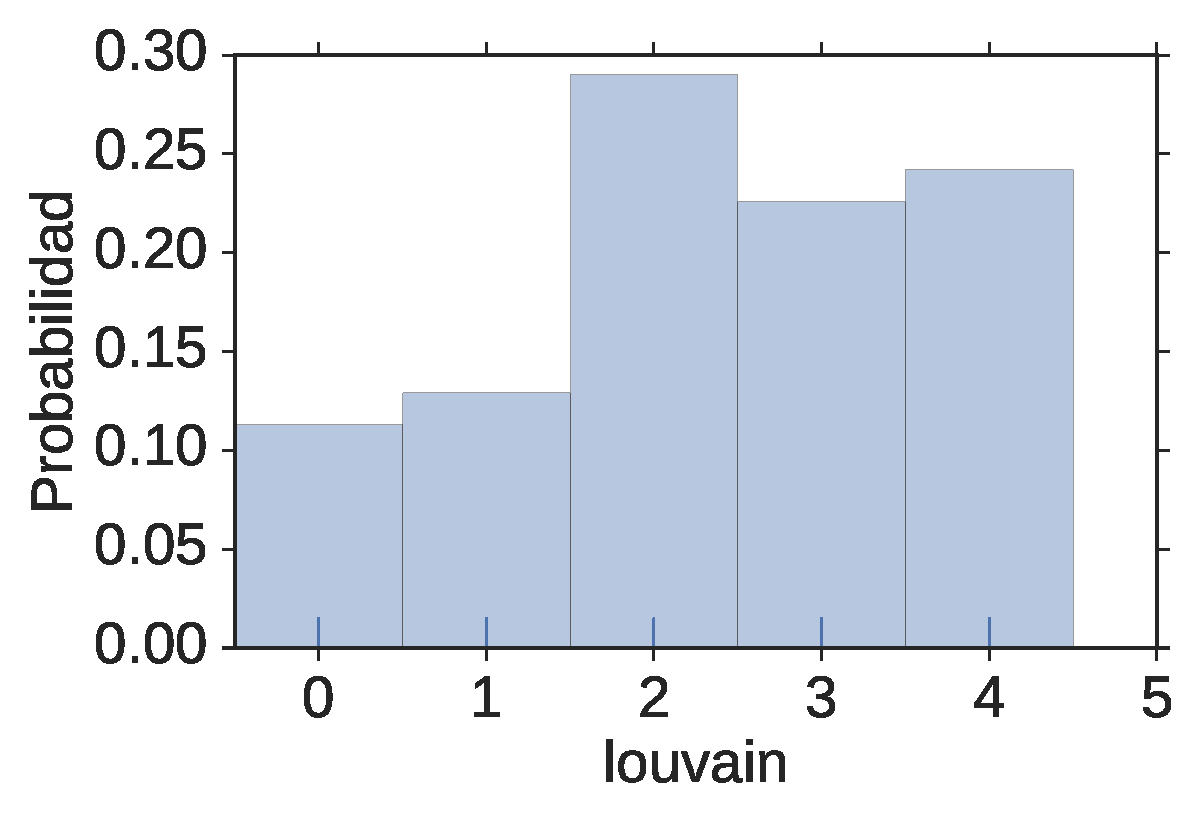
\includegraphics[width=0.95\columnwidth]{figuras/louvain_probability.pdf}
    \end{subfigure}
    \begin{subfigure}[b]{.45\columnwidth}
        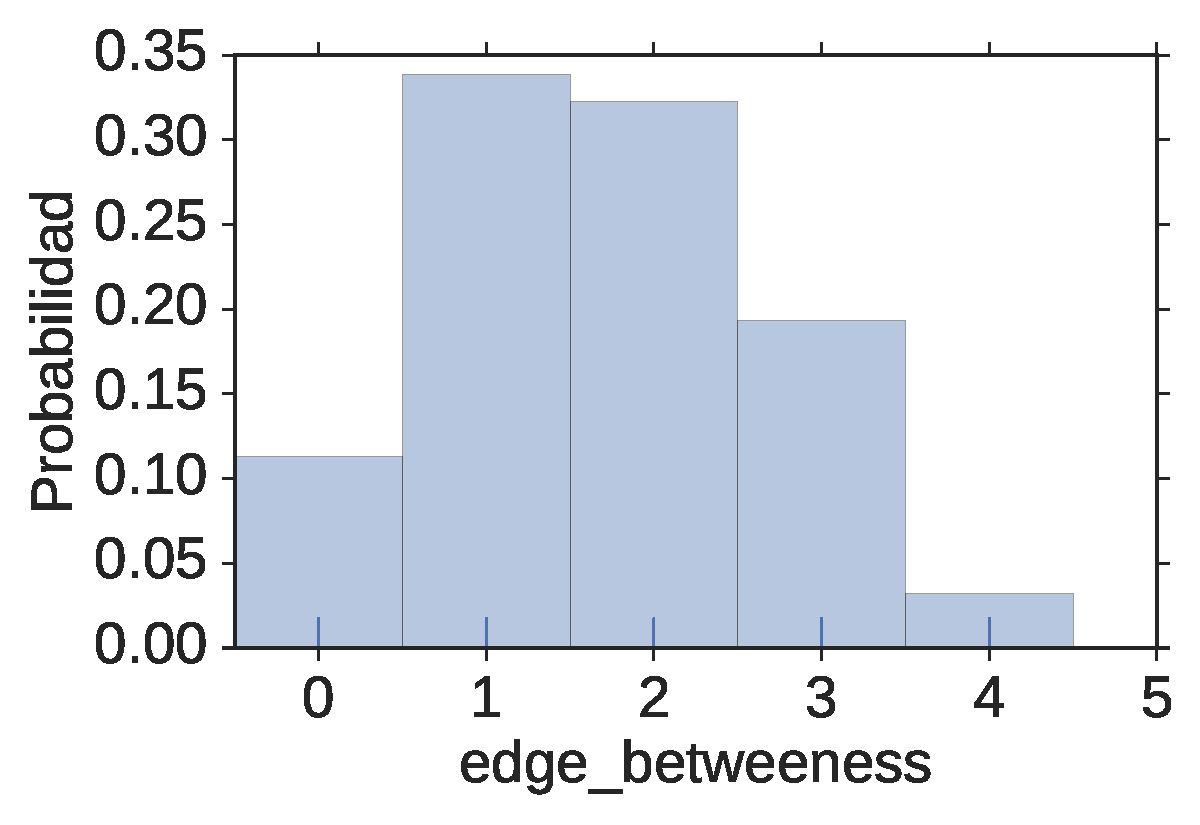
\includegraphics[width=0.95\columnwidth]{figuras/edge_betweeness_probability.pdf}
    \end{subfigure}\\
    \begin{subfigure}[b]{.45\columnwidth}
        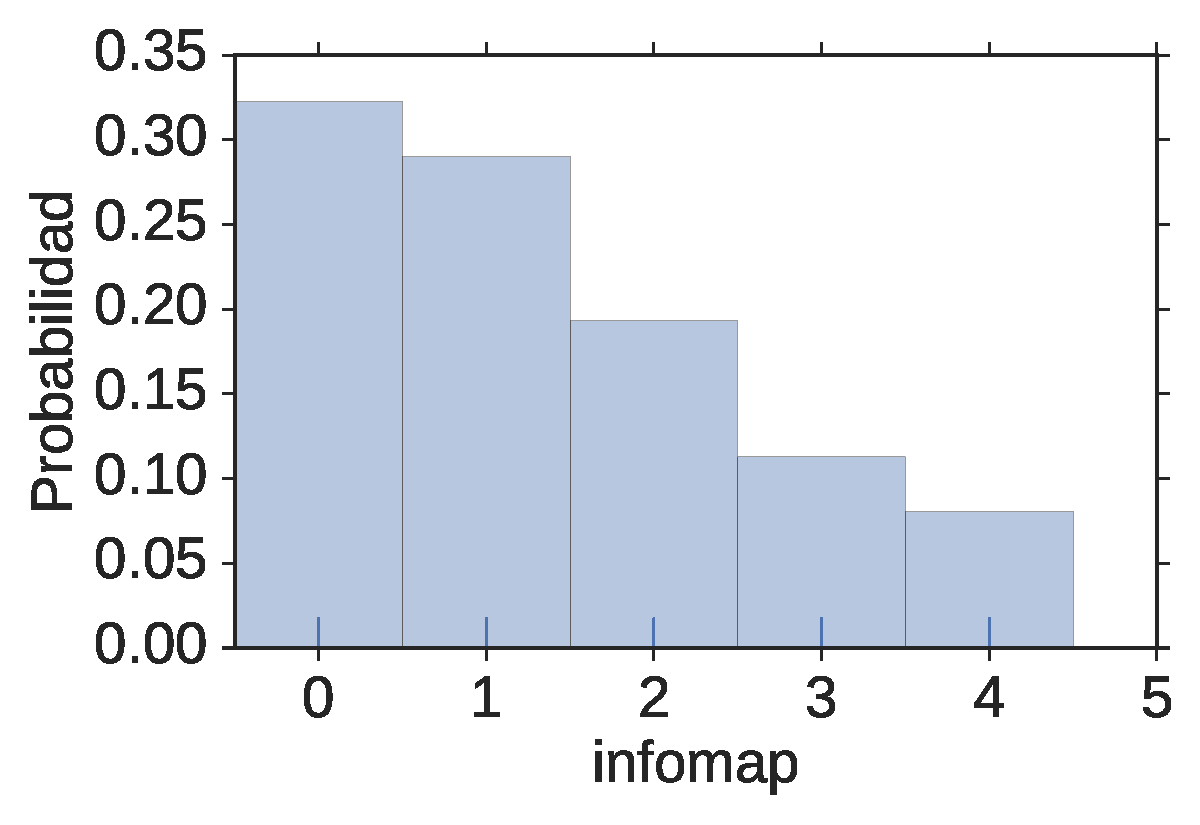
\includegraphics[width=0.95\columnwidth]{figuras/infomap_probability.pdf}
    \end{subfigure}
    \begin{subfigure}[b]{.45\columnwidth}
        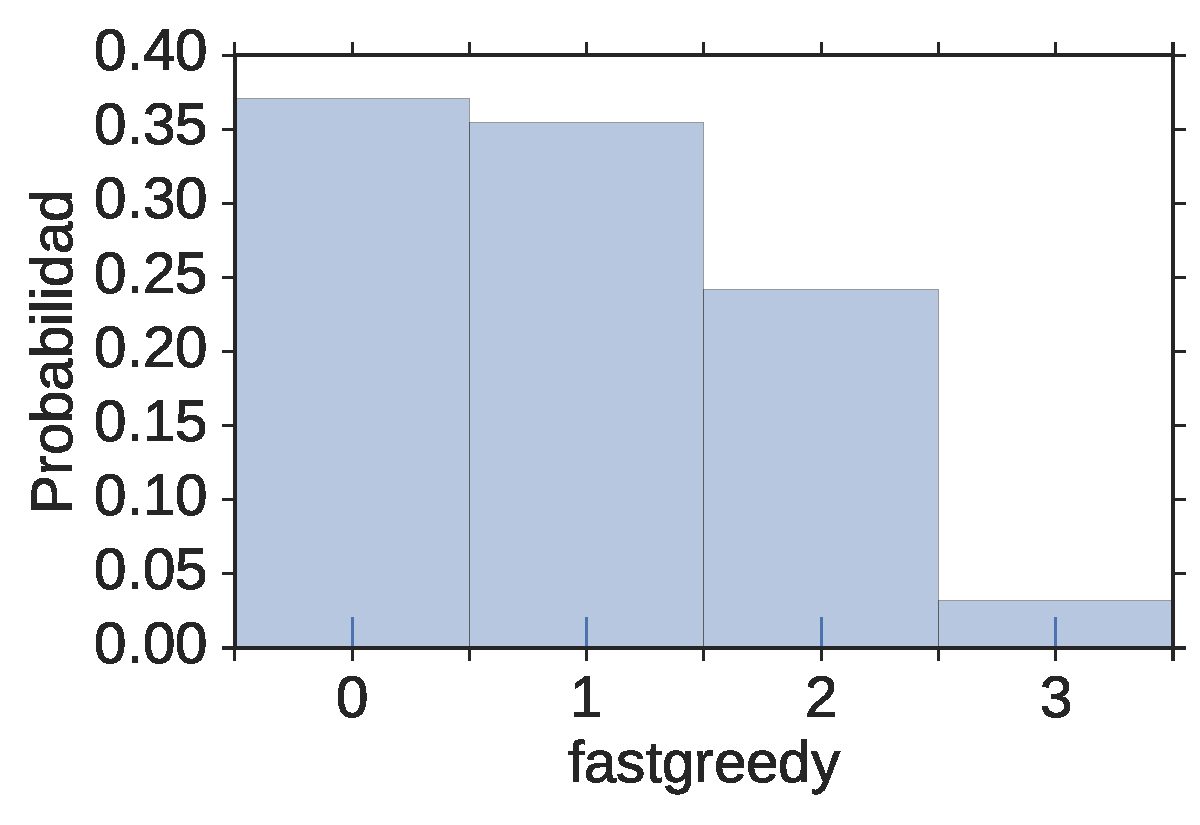
\includegraphics[width=0.95\columnwidth]{figuras/fastgreedy_probability.pdf}
    \end{subfigure}
    \caption{\label{fig:histos} Distribuci\'on de probabilidad de pertenencia de un nodo a una comunidad 
para los diferentes algoritmos utilizados.}
\end{figure}




\begin{figure}[!ht]
    \centering
    \begin{subfigure}[b]{.45\columnwidth}
        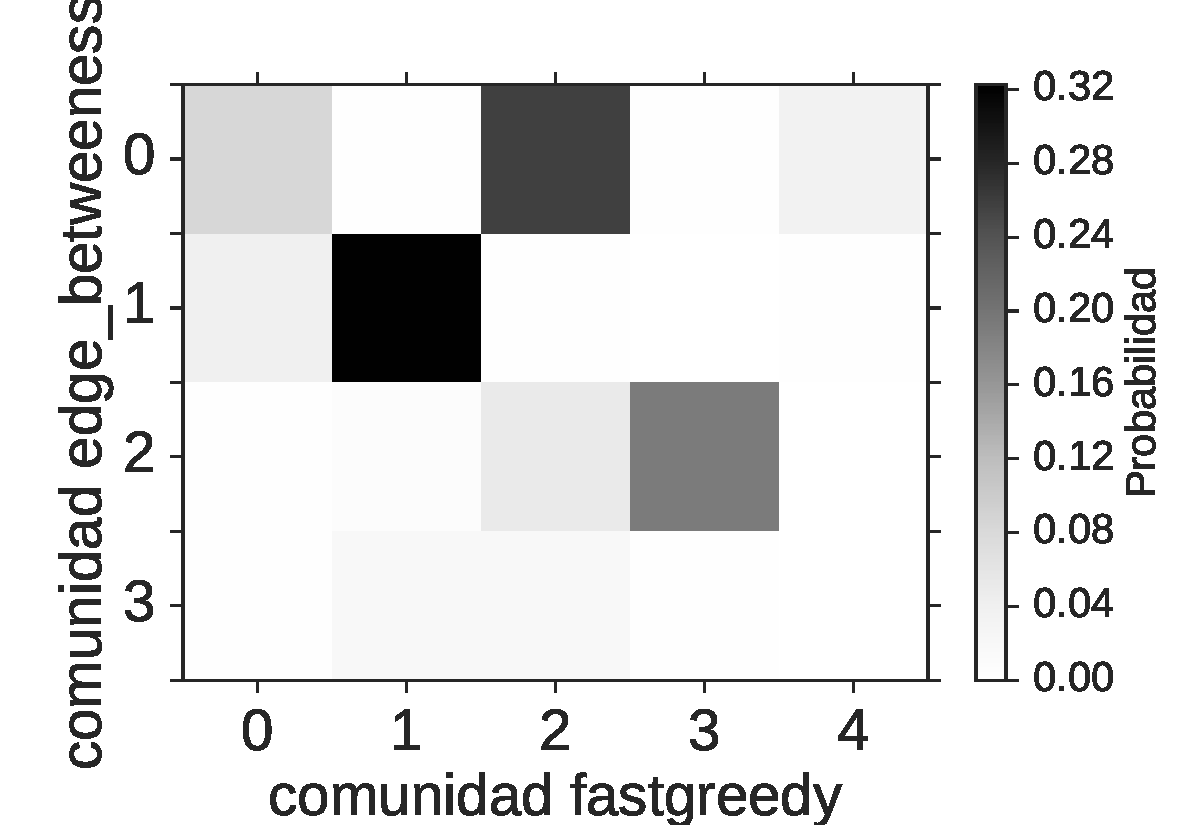
\includegraphics[width=0.95\columnwidth]{figuras/join_proba_fastgreedy-edge_betweeness.pdf}
    \end{subfigure}
    \begin{subfigure}[b]{.45\columnwidth}
        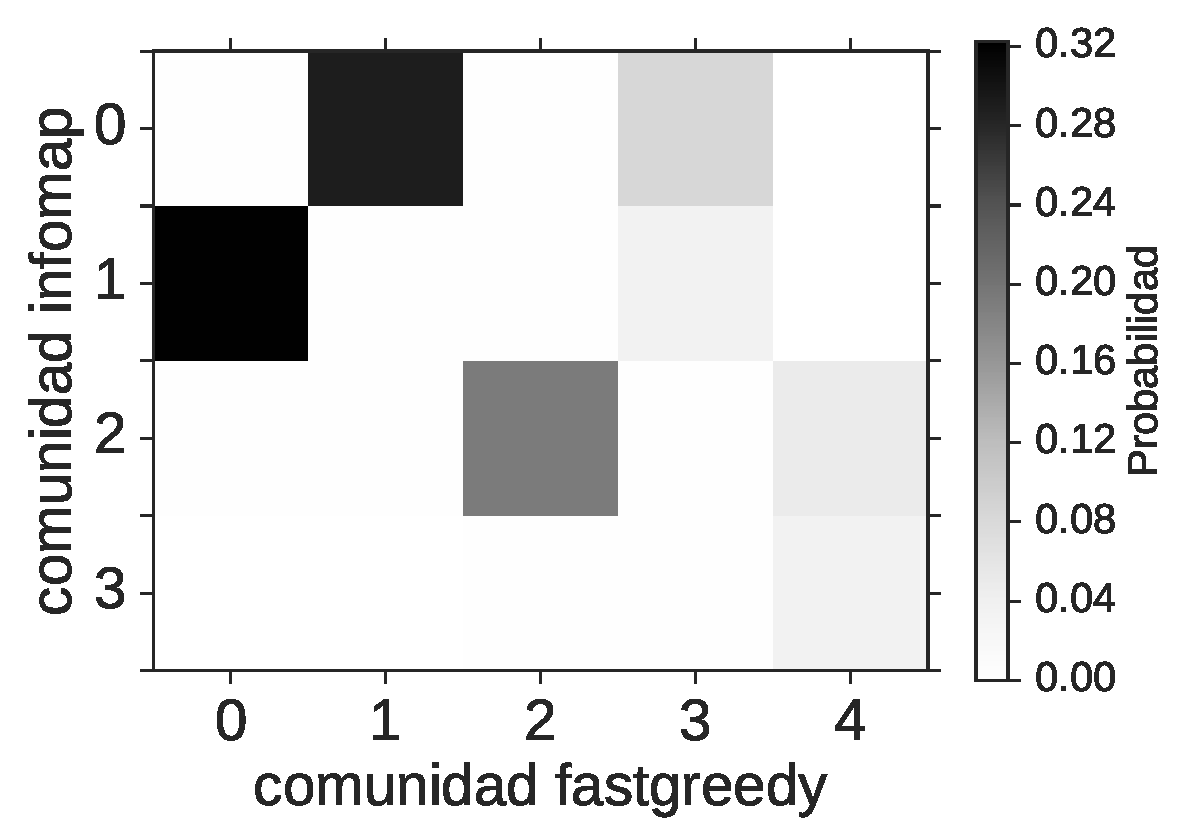
\includegraphics[width=0.95\columnwidth]{figuras/join_proba_fastgreedy-infomap.pdf}
    \end{subfigure}\\
    \begin{subfigure}[b]{.45\columnwidth}
        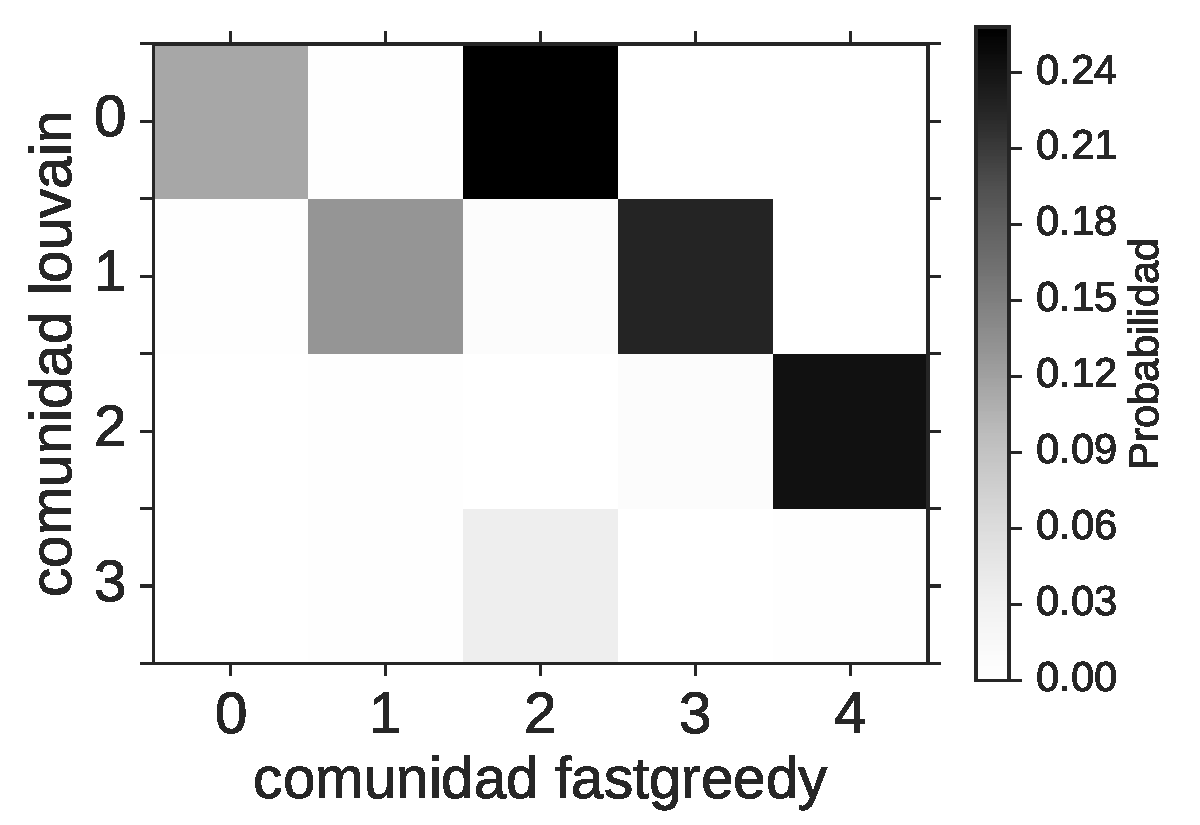
\includegraphics[width=0.95\columnwidth]{figuras/join_proba_fastgreedy-louvain.pdf}
    \end{subfigure}
    \begin{subfigure}[b]{.45\columnwidth}
        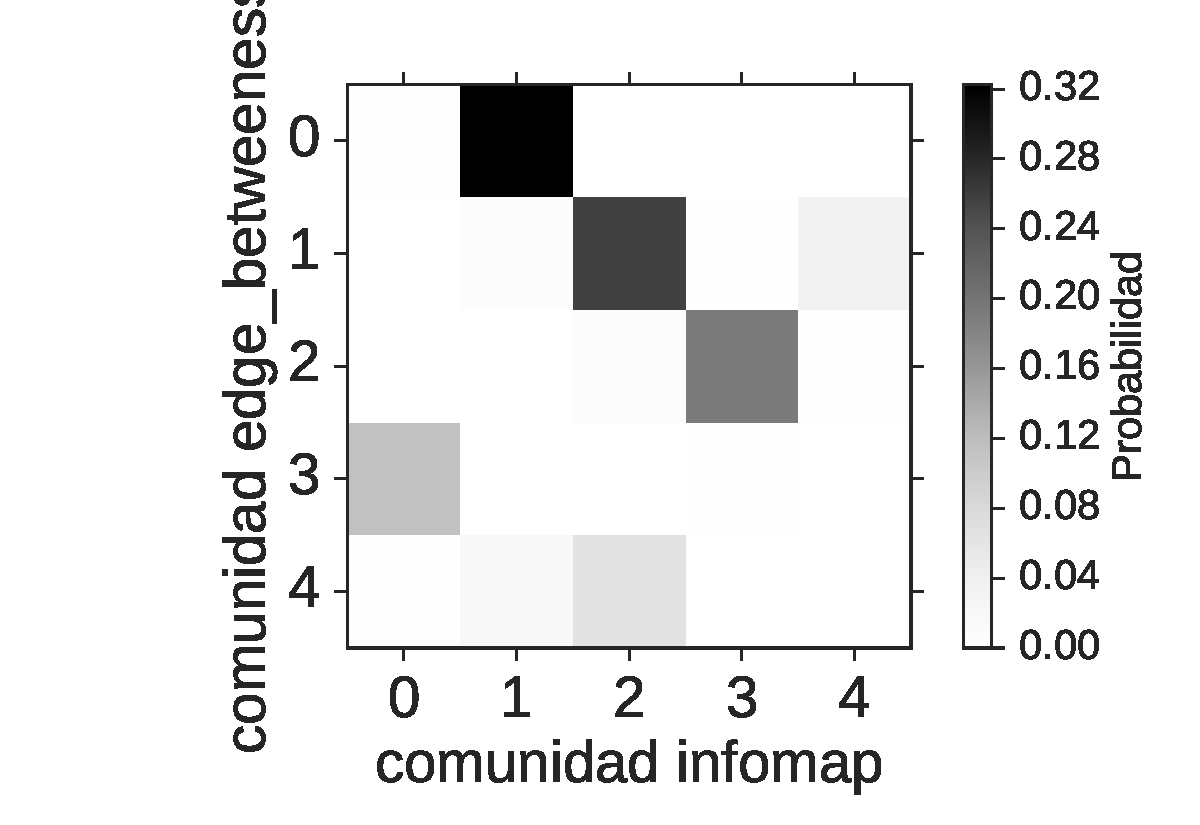
\includegraphics[width=0.95\columnwidth]{figuras/join_proba_infomap-edge_betweeness.pdf}
    \end{subfigure}\\
    \begin{subfigure}[b]{.45\columnwidth}
        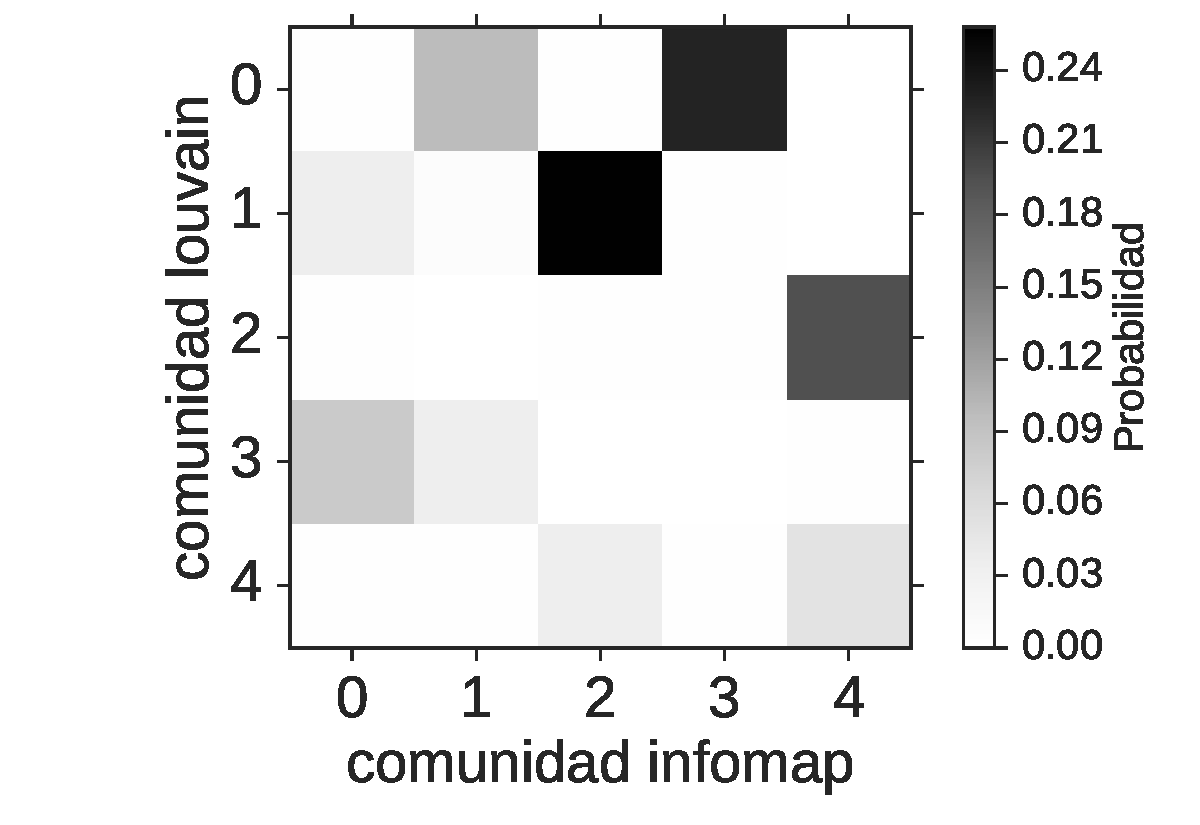
\includegraphics[width=0.95\columnwidth]{figuras/join_proba_infomap-louvain.pdf}
    \end{subfigure}
    \begin{subfigure}[b]{.45\columnwidth}
        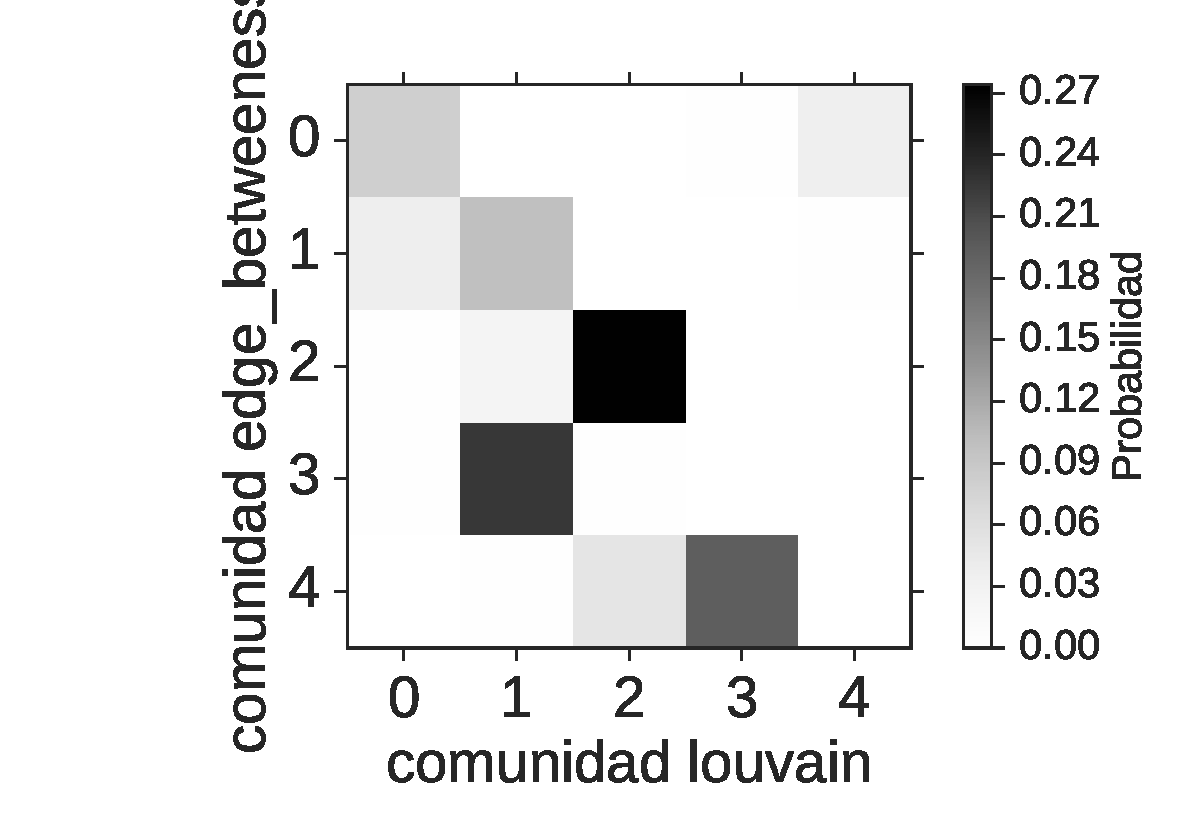
\includegraphics[width=0.95\columnwidth]{figuras/join_proba_louvain-edge_betweeness.pdf}
    \end{subfigure}
    \caption{\label{fig:matrix} Distribuci\'on de probabilidad conjunta de pertenencia de un nodo a una comunidad 
de cada par de algotirmos.}
\end{figure}

La \textit{Informaci\'on Mutua} total, normalizada, es mostrada en la 
Tabla \ref{tab:mi} de la cual se puede observar que los algoritmos {\it infomap}
y {\it louvain} son los m\'as similares con una semejanza del $86.2\%$,  
las rutinas {\it Fast Greedy} y {\it Edge Betweeness} muestran la menor correlaci\'on
con una similitud del $66.2\%$ mientras que en general el resto coinciden en un rango 
de $70\%-80\%$


\begin{table}[!h]
    \centering
    \caption{\label{tab:mi} Informaci\'on mutua entre las particiones encontradas por cada algoritmo.}
    {\scriptsize
    \begin{tabularx}{0.9\textwidth}{Xl|ccccX}
        \hline\hline
        &                 &  Fast Greedy    & Edge betweeness   & Infomap   & Louvain &  \\
        \hline
        & Fast Greedy     & 1.000           & 0.662             & 0.767     & 0.794 \\
        & Edge Betweeness &                 & 1.000             & 0.771     & 0.732 \\
        & Infomap         &                 &                   & 1.000     & 0.862 \\
        & Louvain         &                 &                   &           & 1.000 \\
        \hline\hline
    \end{tabularx}
    }
\end{table}


